\chapter{Fase 3: modelo de datos y contrato de la API}\label{cap:fase3}

\section{Enfoque contract-first}

Escribimos el contrato antes que el código. El archivo \texttt{contracts/openapi.yaml} (OpenAPI~3.1) es la única fuente de verdad entre el frontend y el backend: los DTOs de validación del backend, los tipos del frontend y las pruebas siguen su forma. El contrato se valida con Redocly en cada ejecución del pipeline y se publica con Swagger UI junto con la API, en \texttt{http://3.151.57.252/docs/} (Figura~\ref{fig:swagger}).

\begin{figure}[H]
\centering
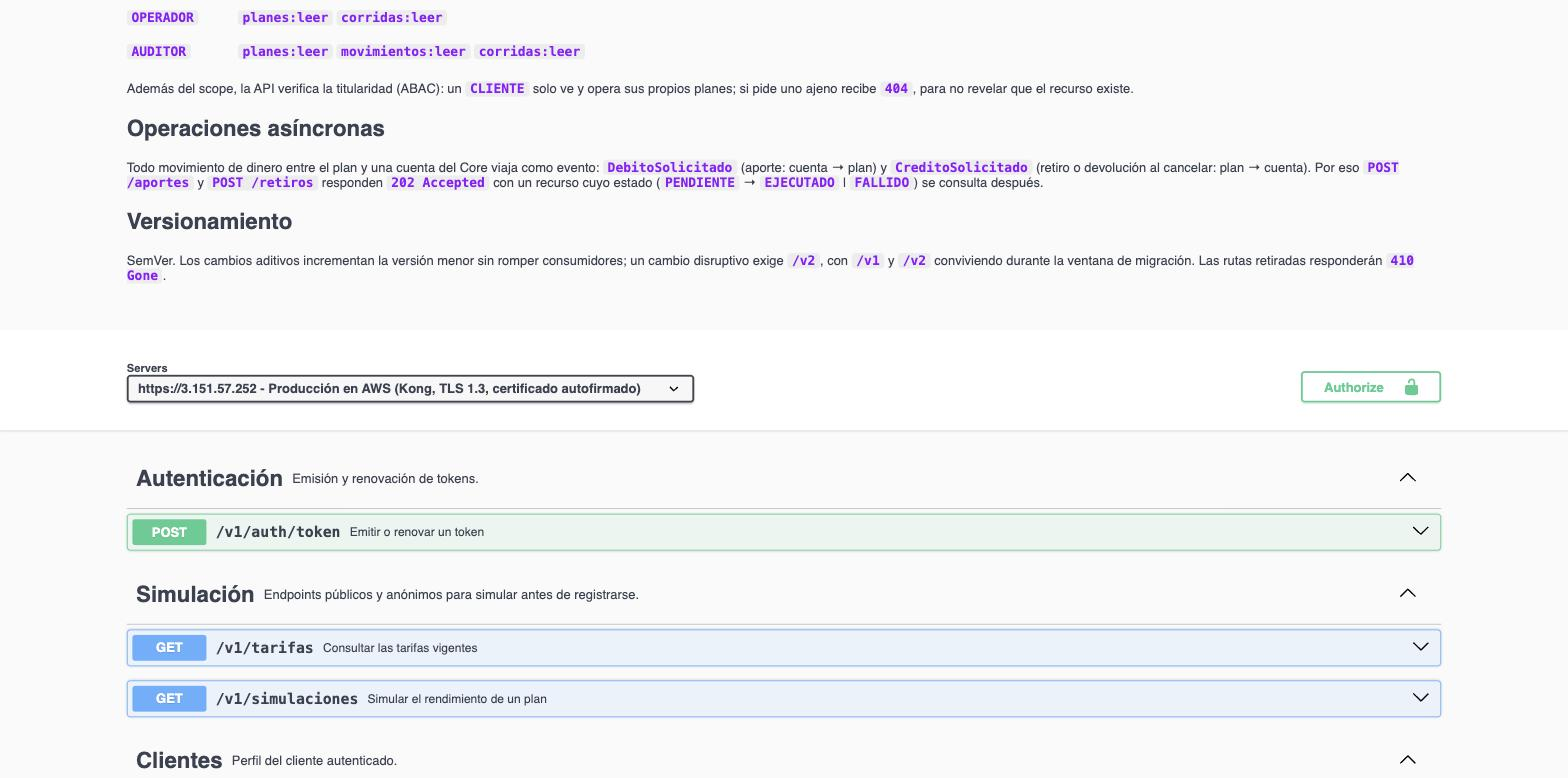
\includegraphics[width=\linewidth]{../evidencias/fase-3-contrato/swagger-ui-endpoints.jpg}
\caption{Contrato publicado con Swagger UI en el entorno de AWS}\label{fig:swagger}
\end{figure}

\section{Convenciones del contrato}

\begin{table}[H]
\centering
\caption{Convenciones de diseño del contrato}\label{tab:convenciones}
\begin{tabularx}{\linewidth}{@{}>{\raggedright}p{3.2cm} X@{}}
\toprule
\textbf{Aspecto} & \textbf{Decisión} \\
\midrule
Rutas & Sustantivos en plural y versión mayor en la ruta (\texttt{/v1}). Las acciones que no son CRUD son sub-recursos (\texttt{/bloqueo}, \texttt{/desbloqueo}, \texttt{/cancelacion}, \texttt{/aportes}, \texttt{/retiros}). No hay \texttt{DELETE}: el historial financiero no se borra. \\
Montos & Enteros en centavos (\texttt{*Centavos}) junto con el código ISO~4217; nunca decimales para dinero. \\
Fechas & ISO~8601: \texttt{date} para fechas de calendario y \texttt{date-time} en UTC para instantes. \\
Errores & \texttt{application/problem+json} (RFC~9457) con un \texttt{codigo} estable para el consumidor. \\
Paginación & Offset (\texttt{pagina}, \texttt{limite}) en planes, cuotas y corridas; cursor opaco (\texttt{cursor}, \texttt{limite}) en movimientos, que crecen sin límite. \\
Operaciones asíncronas & Aportes y retiros responden \texttt{202 Accepted} con un recurso cuyo estado (\texttt{PENDIENTE}, \texttt{EJECUTADO}, \texttt{FALLIDO}) se consulta en \texttt{Location}. \\
Concurrencia & \texttt{Idempotency-Key} en las operaciones que mueven dinero; \texttt{ETag}/\texttt{If-Match} al modificar un plan (412 si cambió). \\
Seguridad & Esquema \texttt{bearerAuth} (JWT); cada operación declara los scopes que exige. \\
Versionamiento & SemVer: los cambios aditivos suben la versión menor; un cambio disruptivo exige \texttt{/v2}. \\
\bottomrule
\end{tabularx}
\end{table}

\section{Modelo de datos orientado a la API}

El modelo que expone la API no copia las tablas de la base de datos: representa lo que el consumidor necesita. Por ejemplo, el saldo del plan no se almacena, se calcula desde el ledger; el progreso es un campo calculado; y la cuenta de débito viaja enmascarada. La Tabla~\ref{tab:recursos} resume los recursos.

\begin{table}[H]
\centering
\caption{Recursos del modelo de la API}\label{tab:recursos}
\begin{tabularx}{\linewidth}{@{}>{\ttfamily\raggedright}p{3.1cm} X@{}}
\toprule
\normalfont\textbf{Recurso} & \textbf{Contenido y reglas} \\
\midrule
PlanAhorro & Meta y fecha objetivo, cuota calculada, plazo y prórrogas, día de débito, cuenta, bloqueo, tasas (TNA base, bono, total y TEA), saldo y saldo disponible derivados del ledger, intereses devengados, progreso, estado (\texttt{ACTIVO}, \texttt{COMPLETADO}, \texttt{CANCELADO}). \\
Simulacion & Cuota mensual, total aportado, intereses proyectados, monto final y proyección mes a mes. Pública y cacheable. \\
TablaTarifas & Tramos de tasa por plazo y bono por bloqueo. \\
Cuota & Calendario de débitos con estado (\texttt{PROGRAMADA}, \texttt{PENDIENTE}, \texttt{EJECUTADA}, \texttt{CANCELADA}) e intentos (máximo 5). \\
Aporte / Retiro & Movimiento de dinero asíncrono con la cuenta del Core, su estado, el motivo de fallo y el \texttt{correlationId}. \\
Movimiento & Asiento del ledger de solo inserción, con el saldo resultante. \\
CuentaDebito & Cuenta del cliente en el Core, enmascarada, con su saldo disponible. \\
CorridaCobro & Resultado de cada corte diario del Batch (para operación y auditoría). \\
Cliente / Token & Perfil del cliente y par de tokens JWT. \\
Problema & Detalle de error RFC~9457 con \texttt{codigo} y errores por campo. \\
\bottomrule
\end{tabularx}
\end{table}

La persistencia, en cambio, está normalizada en PostgreSQL: \texttt{planes}, \texttt{cuotas}, \texttt{operaciones\_core}, el ledger \texttt{movimientos} (protegido por un trigger que rechaza UPDATE y DELETE), \texttt{outbox}, \texttt{eventos\_procesados}, \texttt{idempotencia} y \texttt{corridas\_cobro}. La vista \texttt{vw\_planes} deriva el saldo, los intereses y el monto reservado por retiros pendientes, y el procedimiento \texttt{sp\_procesar\_debitos\_ahorro\_programado} solo selecciona las cuotas a cobrar.

\section{Operaciones del contrato}

La Tabla~\ref{tab:endpoints} lista las 20 operaciones del contrato con el scope que exige cada una y los códigos de estado que documenta. Se genera automáticamente desde el archivo OpenAPI, así que no puede quedar desactualizada respecto del contrato.

\input{generados/fase3-endpoints}

\section{Ajuste del contrato al frontend}

Al revisar el frontend que construyó el equipo, ajustamos el contrato y el alcance: el login pasó a ser por email; la creación del plan usa una fecha objetivo y el sistema calcula la cuota; se agregaron el retiro parcial (RF-04.3) y el desbloqueo con pérdida de los intereses devengados (RF-01.7), con el evento \texttt{CreditoSolicitado} simétrico al débito; y se incorporaron el perfil del cliente, el saldo de las cuentas y un resumen de totales en el listado de planes. Estos cambios se reflejaron en los requerimientos, en la Fase~2 y en el diagrama C4.

\section{Validación}

El contrato se valida con Redocly sin errores (Anexo~\ref{anx:evidencias}). Las dos advertencias restantes corresponden a la URL de servidor local (\texttt{localhost}), que se mantiene a propósito para el entorno de desarrollo.
